

% You may title this section "Methods" or "Models". 
% "Models" is not a valid title for PLoS ONE authors. However, PLoS ONE
% authors may use "Analysis" 
\section{Models}

\begin{figure}[h!]
\centering
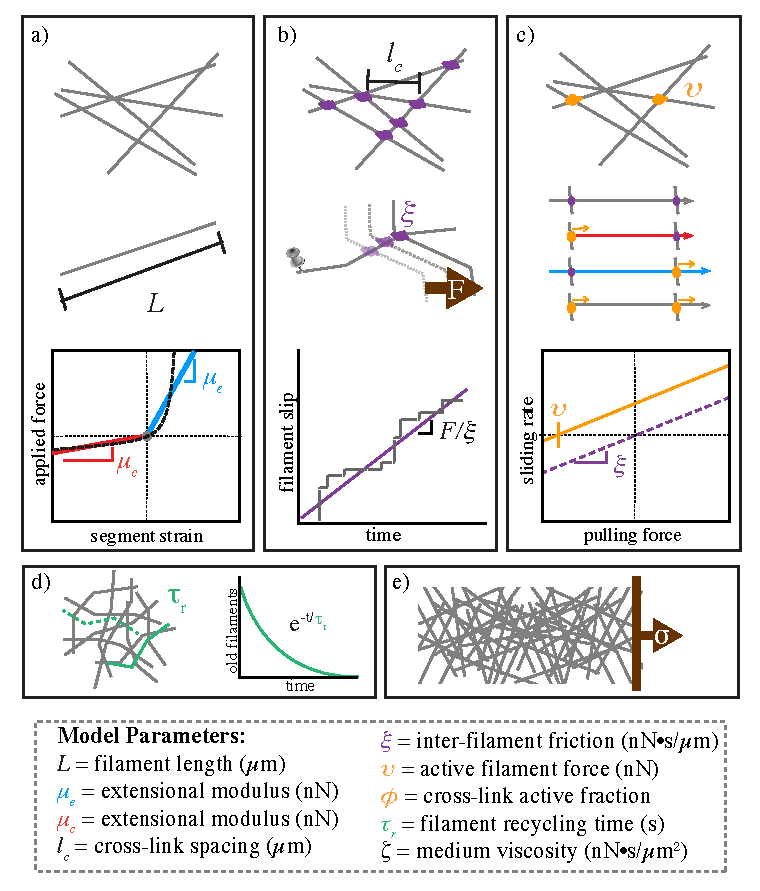
\includegraphics[width=\hsize]{model/figures/fig2/fig2}
\caption{\label{fig:sim} Schematic of modeling framework. a) Asymmetric filament compliance.Filaments have smaller spring constant for compression than for extension. b) Cross-link slip. Cross-links are coupled by an effective drag, such that their relative motion is
proportional to any applied force. c) Motor activity. Filament activity manifests as a basal sliding rate even in the absence of an external force. Fractional activity. Only a subset of filament cross-links are active, resulting in differential force exertion along the filament. d) Filament recycling. Filaments are turned over at a constant rate, leading to a refreshing in the strain state of all filaments after a characteristic timescale. e) Applied stress. In simulations with passive cross-links, and external stress is applied as force filed acting on a fixed spatial domain.}
\end{figure}

Our motivation is to model essential microscope features of cross-linked actomyosin networks (semi flexible actin filaments with asymmetric compliance, dynamic cross-links, active motors and and continuous filament recycling), in a way that is simple enough to allow systematic exploration of how tuning these microscopic features controls macroscopic network deformation and flow. We focus on 2D networks for computational tractability and because they capture a reasonable approximation of the quasi-2D cortical actomyosin networks that govern flow and deformation in many eukaryotic cells\cite{cellmech_flows, salbreuxbphs}, or the quasi-2D networks studied recently in vitro\cite{rheo_2D1,rheo_2D2}.


\subsection{Asymmetric filament compliance}
We model individual filaments as chains of springs with relaxed length $l_s$.  Filaments can therefore be represented as a sequence of nodes with positions $\mathbf{x_i}$, where the index $i$ enumerates over all nodes of all segments.  The internal elastic resistance of filament segments gives rise to nearest neighbor force interactions, $\mathbf{F^{\mu}_{i,i+1}}$, of the form

\begin{equation}
\label{eqn:spring}
\mathbf{F^{\mu}_{i,i+1}} = \mu\frac{|\mathbf{x_{i+1}}-\mathbf{x_i}|-l_s}{l_s}\left ( \frac{\mathbf{x_{i+1}}-\mathbf{x_i}}{l_s}\right )
\end{equation}


where the modulus, $\mu$, is a composite quantity representing both filament and cross-linker compliance in a manner similar to a proposed effective medium theory \cite{theo_crosslinknonlinear}. To model asymmetric filament compliance, we assign a different value to the modulus $\mu$,  depending on whether the strain on a given filament segment, $(|\mathbf{x_{i-1}}-\mathbf{x_i}|-l_s)/l_s$, is greater or less than 0. In the limit of highly rigid cross-links and flexible filaments, our model reduces to the pure semi-flexible filament models of \cite{theo_hlm,theo_hlm2}. In the opposite regime of nearly rigid filaments and highly flexible cross links, our model is essentially the same as that of \cite{theo_crosslinknonlinear} in small strain regimes before any nonlinear cross link stiffening. In a departure from those previous models, we assume here that the magnitude of the force on interior cross-links is the same as those on the exterior. This approach ignores the variation in strain on these two sets of cross-links as addressed in \cite{theo_crosslinknonlinear}, but we choose to ignore this variation in favor of an approximated, global mean approach. 

Because we are dealing with semi-flexible filaments we also introduce a bending modulus between our filament segments such that the restoring force is proportional to the angle between the filament segments and points in the direction orthogonal to the filament direction, $\mathbf{u_i}=(\mathbf{x_{i-1}}-\mathbf{x_{i}})/|\mathbf{x_{i-1}}-\mathbf{x_{i}}|$.   


The total internal force on a filament node i can therefore be written as:

\begin{equation}
\label{eqn:internal}
\mathbf{F^{int}_i} = \mathbf{F^{\mu}_{i-1,i}} + \mathbf{F^{\mu}_{i,i+1}} 
\end{equation}

Introducing a filament bending stiffness adds another mode of asymmetric compliance since filaments can bend/buckle internally under compression. For the majority of the work presented here, we have set $l_s=L$ to obviate dependence on bending driven asymmetries. However, as shown in supplemental figure xxx (TBA)  the major points of the paper are still valid for $l_s<L$ under the condition that $\kappa/l_s\gg\mu_c$. 

\subsection{Drag-like coupling between overlapping filaments}
\label{exp_drag}
Previous models represent cross-linkers as elastic connections between pairs of points on neighboring filaments that appear and disappear with either fixed or force-dependent probabilities \cite{model_taeyoon,theo_crosslinknonlinear}.  Here, we introduce a simpler coarse-grained model for dynamic cross-links by replacing many transient elastic interactions with an effective drag-like coupling between every pair of overlapping segments.
\begin{equation}
\label{eqn:drag}
\mathbf{F^{\xi}_{i-1,i}} = \xi \sum_j \frac{l_s-|s_{ij}-s_i|}{l_s}  (\mathbf{v_{i-1,i}}-\mathbf{v_{j-1,j}}) 
\end{equation}

where $\mathbf{v_{n-1,n}}$ represent the average velocity of the filament segment spanning nodes $n-1$ and $n$, and the sum is taken over all filament segments such that the segment from node $j-1$ to node $j$ intersects the segment from $i-1$ to $i$ at the location $s_{ij}$.

\begin{equation}
\label{eqn:drag}
\mathbf{F^{coup}_{i}} = \mathbf{F^{\xi}_{i-1,i}} + \mathbf{F^{\xi}_{i,i-1}} 
\end{equation}

This model assumes a linear relation between the drag force and the velocity difference between attached segments.  This drag-like coupling has been shown to be an adequate approximation in the case of ionic cross-linking of actin\cite{mol_fric,theo_hydroish2}, and can be found in the theoretical basis of force-velocity curves for myosin bound filaments\cite{theo_frictionShila}. Although non-linearities can arise through force dependent detachment kinetics and/or non-linear force extension of cross-links, we assume that inhomogeneities from non-linear effects are of second or higher order. With this assumption, the motion of filaments can be described by a deterministic dynamical equation of the form

\begin{equation}
\label{eqn:syst1}
0 = -l_s\zeta\mathbf{ v_i} -\mathbf{F^{coup}_i}+ \mathbf{F^{int}_i}
\end{equation}

Here, the first term is the filament's intrinsic drag through its embedding fluid, $\zeta$, while the second comes from the drag-like coupling between filaments, $\xi$.  

\subsection{Active coupling for motor driven filament interactions}

To add motor activity we select a subset of cross-linked points and impose an additional force of magnitude $\upsilon$ on each of the overlapping filament segments, directed towards the (+) end of that segment, $\mathbf{u_i}=(\mathbf{x_{i-1}}-\mathbf{x_{i}})/|\mathbf{x_{i-1}}-\mathbf{x_{i}}|$. Thus, the total ``active'' force on a given filament segment is

\begin{equation}
\label{eqn:moto}
\mathbf{F^{\upsilon}_{i-1,i}}=\upsilon \mathbf{u_i}\sum_j \frac{l_s-|s_{ij}-s_i|}{l_s}q_{ij}
\end{equation}

where $q_{ij}$ equals 0 or 1 depending on whether there is an ``active'' cross-linker at this location. To model dispersion of motor activity, we  set $q_{ij}=1$  on a randomly selected subset of cross-link points, such that $\bar{q}=\phi$, where $\bar{q}$ indicates the mean of $q$.



Finally, for each active force, $\mathbf{F^{act}_j}$, imparted by filament $j$, we must also impart the opposite force onto the filament between $i$ and $i+1$ as well.  Therefore, the entire equation for activity will appear as

\begin{equation}
\label{eqn:active}
\mathbf{F^{act}_{i}}=\mathbf{F^{\upsilon}_{i-1,i}} + \mathbf{F^{\upsilon}_{i,i+1}}
- \sum_{j}\mathbf{F^{\upsilon}_{j-1,j}}q_{ij}
\end{equation}


This will leave us with a full equation of motion given by the sum of each of the parts defined above.

\begin{equation}
\label{eqn:syst3}
0=-L\zeta\mathbf{ v_i} -\mathbf{F^{coup}_i}+ \mathbf{F^{int}_i}+\mathbf{F^{act}_i} 
\end{equation}

\subsection{2D network formation}

We used a mikado model approach \cite{Unterberger2014} to initialize a minimal network of connected unstressed linear filaments in a rectangular 2D domain. We generate 2D networks of these semi-flexible filaments by laying down straight lines of length, L, with random position and orientation. We then assume that overlapping filaments become cross-linked at their points of overlap. Although real cytoskeletal networks may form with non-negligible anisotropy, for simplicity, we focus on isotropically initialized networks. We define the density using the average distance between cross-links along a filament, $l_c$. A simple geometrical argument can then be used to derive the number of filaments filling a domain as a function of $L$ and $l_c$\cite{theo_hlm}.  Here, we use the approximation that the number of filaments needed to tile a rectangular domain of size $D_x \times D_y$  is $2D_xD_y/Ll_c$, and that the length density is therefore simply, $2/l_c$. In the absence of cross-link slip, we expect the network to form a connected solid with a well defined elastic modulus\cite{theo_hlm,theo_hlm2}.


\subsection{External applied stress}
We can model our active networks as a coupled system of differential equations satisfying \ref{eqn:syst3}.  However, to probe the passive response of the network, we also wish to incorporate externally applied stresses.  Although the general passive mechanical response of this system may be very complex, we focus our attention on low frequency deformations and the steady-state creep response of the system to an applied stress.  To do this we introduce a fixed stress, $\sigma$ along a fixed domain at one edge of the network.  The stress is applied via individual forces to the filaments lying within a patch of size $D_w$ such that the sum of individual forces is equal to the applied stress times the height of the domain.  These forces point in the direction, $\mathbf{\hat{x}}$, producing an extension of the patch.  The region of applied stress does not move as the network deforms, allowing us to more easily focus our attention on a fixed sized domain. 

Finally, we add a 0 velocity constraint at the other edge of our domain of interest.  We assume that our network is in the ``dry,'' low Reynold's number limit, where inertial effects are so small that we can equate our total force to 0.  Therefore, we have a dynamical system of wormlike chain filaments satisfying

\begin{equation}
\label{eqn:systfull}
0=-L\zeta\mathbf{ v_i} -\mathbf{F^{coup}_i}+ \mathbf{F^{int}_i}+\mathbf{F^{act}_i} + \sigma\mathbf{\hat{u}(x_i)}
\end{equation}

subject to constraints such that $\mathbf{v_i(x)}$ is 0 with $x=0$.  This results in an implicit differential equation for filament segments which can be discretized and integrated in time to produce a solution for the motion of the system.


\subsection{Modeling filament turnover}

In living cells, actin filament assembly is governed by multiple factors that control nucleation, elongation and filament branching. Likewise filament disassembly is governed by multiple factors that promote filament severing and monomer dissociation at filament ends. Here, we focus on a lowest order model for filament recycling in which entire filaments appear with a fixed rate per unit area, $k_{app}$ and disappear at a rate $k_{diss}\rho$, where $\rho$ is a filament density. With this assumption, in the absence of network deformation, the density of filaments will equilibrate to a steady state density, $k_{app}/k_{diss}$, with time constant $\tau_r = 1/k_{diss}$.   In deforming networks, the density will be set by a competition between strain thinning ($\gamma>0$) or thickening ($\gamma<0$), and density equilibration via turnover. To implement this assumption, at fixed time interval $\tau_s < 0.01\cdot\tau_r$ (i.e. 1\% of the equilibration time), we selected a fraction, $\tau_s/\tau_r$, of existing filaments (i.e. less than 1\% of the total filaments) for degradation. We then generated a fixed number of new unstrained filaments $k_{app}\tau_sD_xD_y$ at random positions and orientations within the original domain.   We refer to this continuous turnover as filament recycling, to $k_{diss}=1/\tau_r$ as the recycling rate, and to $\tau_r$ as the recycling time.


\subsection{Simulation methods}

Details of our simulation approach can be found in the Appendix. Briefly, equations \ref{eqn:spring},\ref{eqn:drag},\ref{eqn:moto} and \ref{eqn:systfull} define a coupled system of ordinary differential equations for the velocities of the endpoints of filament segments, $\mathbf{\dot{x}}$.  These equations are coupled by the effective cross-link friction on segment overlap points, yielding a system of the form:

\begin{equation}
\mathbf{A \cdot \dot x} = \mathbf{f(x)}
\end{equation}

where $\mathbf{A }$ represents a coupling matrix between endpoints of filaments that overlap, and $\mathbf{f(x)}$ is the spring force between pairs of filament segment endpoints.   We numerically integrate this system of equations to find the time evolution of the positions of all filament endpoints. We generate a network of filaments with random positions and orientations as described above within a domain of size $D_x$ by $D_y$.  For all simulations, we imposed periodic boundaries in the y-dimension. To impose an extensional stress, we constrained all filament segment endpoints within a fixed distance $0.05\cdot D_x$ from the left edge of the domain to be non-moving, then we imposed a rightwards force on all segment endpoints within a distance $0.05\cdot D_x$ from the left edge of the patch.   To simulate free contraction, we removed all constraints at boundaries; to assess buildup of contractile stress under isometricc conditions, we pinned both left and right edges of the network as described above.




We smoothed all filament interactions, force fields, and constraints over small regions such that the equations contained no sharp discontinuities. The nominal units for length, force, and time are $\mu m$, nN, and s, respectively.  We explored parameter space around an estimate of biologically relevant parameter values given in Table \ref{table:para}. 

\begin{table}[h]
\centering
\caption{Simulation Parameter Values}
\label{table:para}
\begin{tabular}{|c|c|c|c|c|}
\hline
{\bf parameter}             & {\bf symbol} & {\bf physiological estimate}          \\ \hline
extensional modulus         & $\mu_e$        & $1 nN $                                               \\
compressional modulus             & $\mu_c$     & $ 0.01 nN $                           \\
cross-link drag coefficient & $\xi$      & $unknown $              \\
solvent drag coefficient     & $\zeta$        & $0.0005 \frac{nN s}{\mu m^2} $      \\
filament length             & L            & $5 \mu m$                                          \\
cross-link spacing          & $l_c$        & $0.5 \mu m$                                         \\
domain size                 & $D_x\times D_y$            & $20\times 50 \mu m$                                 \\ \hline
\end{tabular}
\end{table}




